\documentclass{article}[18pt]
\ProvidesPackage{format}
%Page setup
\usepackage[utf8]{inputenc}
\usepackage[margin=0.7in]{geometry}
\usepackage{parselines} 
\usepackage[english]{babel}
\usepackage{fancyhdr}
\usepackage{titlesec}
\hyphenpenalty=10000

\pagestyle{fancy}
\fancyhf{}
\rhead{Sam Robbins}
\rfoot{Page \thepage}

%Characters
\usepackage{amsmath}
\usepackage{amssymb}
\usepackage{gensymb}
\newcommand{\R}{\mathbb{R}}

%Diagrams
\usepackage{pgfplots}
\usepackage{graphicx}
\usepackage{tabularx}
\usepackage{relsize}
\pgfplotsset{width=10cm,compat=1.9}
\usepackage{float}

%Length Setting
\titlespacing\section{0pt}{14pt plus 4pt minus 2pt}{0pt plus 2pt minus 2pt}
\newlength\tindent
\setlength{\tindent}{\parindent}
\setlength{\parindent}{0pt}
\renewcommand{\indent}{\hspace*{\tindent}}

%Programming Font
\usepackage{courier}
\usepackage{listings}
\usepackage{pxfonts}

%Lists
\usepackage{enumerate}
\usepackage{enumitem}

% Networks Macro
\usepackage{tikz}


% Commands for files converted using pandoc
\providecommand{\tightlist}{%
	\setlength{\itemsep}{0pt}\setlength{\parskip}{0pt}}
\usepackage{hyperref}

% Get nice commands for floor and ceil
\usepackage{mathtools}
\DeclarePairedDelimiter{\ceil}{\lceil}{\rceil}
\DeclarePairedDelimiter{\floor}{\lfloor}{\rfloor}

% Allow itemize to go up to 20 levels deep (just change the number if you need more you madman)
\usepackage{enumitem}
\setlistdepth{20}
\renewlist{itemize}{itemize}{20}

% initially, use dots for all levels
\setlist[itemize]{label=$\cdot$}

% customize the first 3 levels
\setlist[itemize,1]{label=\textbullet}
\setlist[itemize,2]{label=--}
\setlist[itemize,3]{label=*}

% Definition and Important Stuff
% Important stuff
\usepackage[framemethod=TikZ]{mdframed}

\newcounter{theo}[section]\setcounter{theo}{0}
\renewcommand{\thetheo}{\arabic{section}.\arabic{theo}}
\newenvironment{important}[1][]{%
	\refstepcounter{theo}%
	\ifstrempty{#1}%
	{\mdfsetup{%
			frametitle={%
				\tikz[baseline=(current bounding box.east),outer sep=0pt]
				\node[anchor=east,rectangle,fill=red!50]
				{\strut Important};}}
	}%
	{\mdfsetup{%
			frametitle={%
				\tikz[baseline=(current bounding box.east),outer sep=0pt]
				\node[anchor=east,rectangle,fill=red!50]
				{\strut Important:~#1};}}%
	}%
	\mdfsetup{innertopmargin=10pt,linecolor=red!50,%
		linewidth=2pt,topline=true,%
		frametitleaboveskip=\dimexpr-\ht\strutbox\relax
	}
	\begin{mdframed}[]\relax%
		\centering
		}{\end{mdframed}}



\newcounter{lem}[section]\setcounter{lem}{0}
\renewcommand{\thelem}{\arabic{section}.\arabic{lem}}
\newenvironment{defin}[1][]{%
	\refstepcounter{lem}%
	\ifstrempty{#1}%
	{\mdfsetup{%
			frametitle={%
				\tikz[baseline=(current bounding box.east),outer sep=0pt]
				\node[anchor=east,rectangle,fill=blue!20]
				{\strut Definition};}}
	}%
	{\mdfsetup{%
			frametitle={%
				\tikz[baseline=(current bounding box.east),outer sep=0pt]
				\node[anchor=east,rectangle,fill=blue!20]
				{\strut Definition:~#1};}}%
	}%
	\mdfsetup{innertopmargin=10pt,linecolor=blue!20,%
		linewidth=2pt,topline=true,%
		frametitleaboveskip=\dimexpr-\ht\strutbox\relax
	}
	\begin{mdframed}[]\relax%
		\centering
		}{\end{mdframed}}
\lhead{Software Engineering}


\begin{document}
\begin{center}
\underline{\huge Standards}
\end{center}

Why standards?
\begin{itemize}
	\item Quality
	\item Shared communication
	\item Shared understanding
	\item Influence, from understanding to creation/development
	\item Profit
	\item Collaboration
	\item Reputation
	\item Regulation (assurance)
	\item Flexibility
\end{itemize}
Importance
\begin{itemize}
	\item They encapsulate best practice (normally)
	\item Framework for QA
	\item Provide continuity
	\begin{itemize}
		\item Record of decision making process
		\item Organisational memory
		\item New staff save time
	\end{itemize}
\end{itemize}
Issues:
\begin{itemize}
	\item Standards are considered too large, unwieldy and difficult to adopt for SMEs
	\item Focus is on large organisations
	\item Concerns over cost and documentation
	\item Difficult to justify
\end{itemize}
\section{Software standards}
Standards are about providing rules, guidelines and heuristics which, if followed, deliver an assurance of good practice - they are not intended to be about best practice\\
\\
Standards may be international, national, organisational or project standards.\\
\\
\textbf{Product} standards define characteristics that all software components should exhibit\\
\\
\textbf{Process} standards define how the software process should be enacted





\section{ISO SC7}
\subsection{Structure}
\begin{center}
	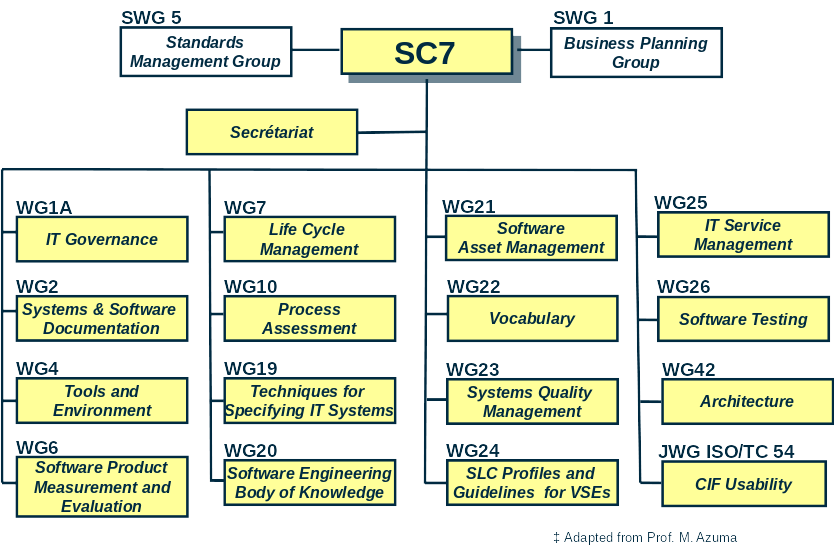
\includegraphics[scale=0.7]{SC7}
\end{center}
\subsection{Domains}
\begin{center}
	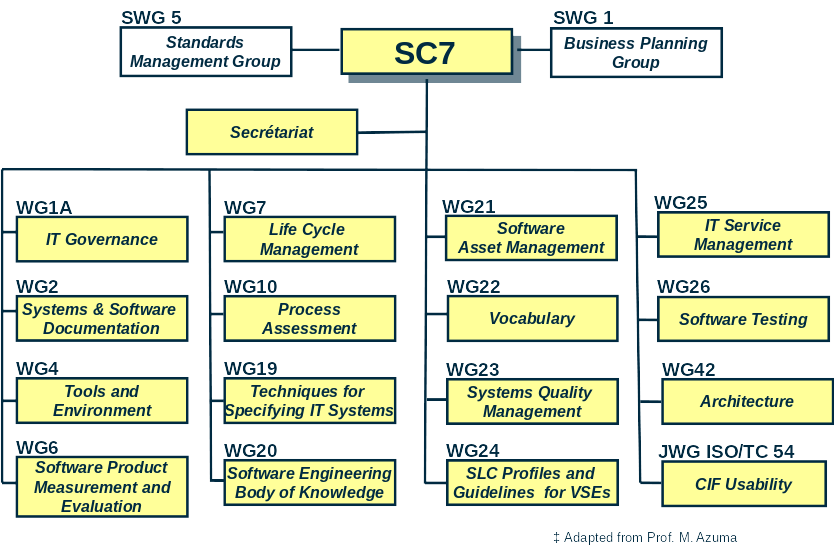
\includegraphics[scale=0.7]{Domains}
\end{center}
\subsection{Standards}
\begin{center}
	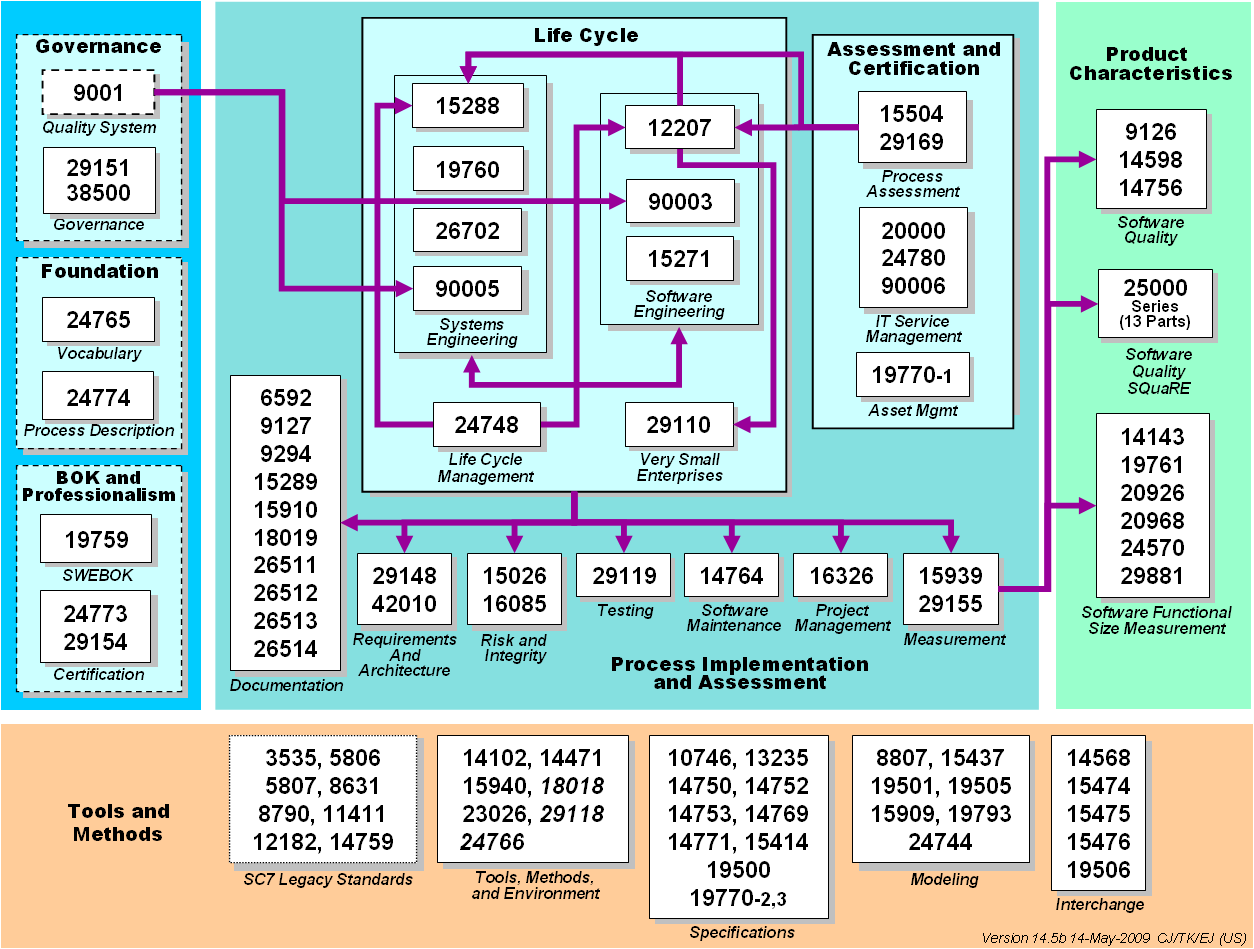
\includegraphics[scale=0.7]{Standards1}
\end{center}
Standards of particular interest
\begin{itemize}
	\item ISO 9000, family of standards for quality management systems
	\item ISO 12207, defines the software engineering process, activity, and tasks that are associated with a software life cycle process from conception through retirement
	\item ISO 15504, also known as SPICE (Software Process Improvement and Capability Determination), is a framework for the assessment of processes
\end{itemize}
\section{ISO 9000}
\begin{center}
	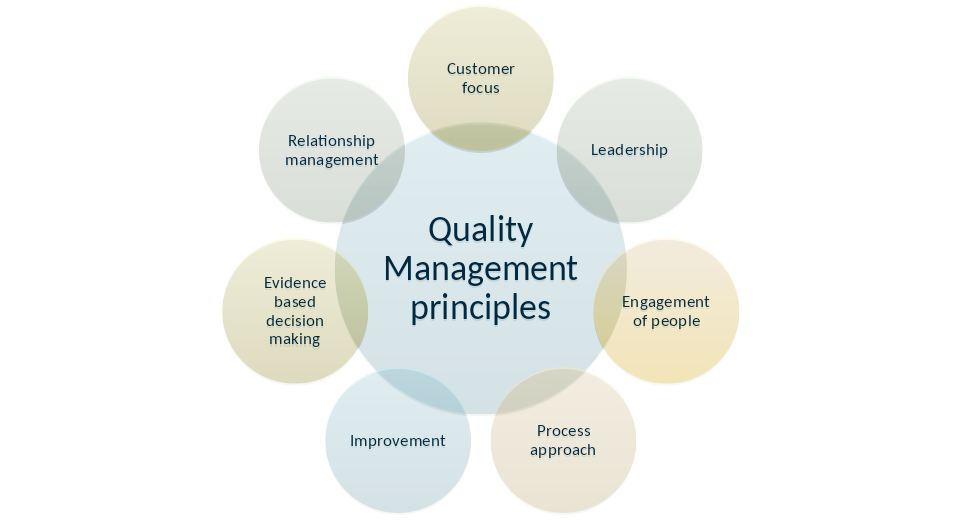
\includegraphics[scale=0.7]{ISO9000}
\end{center}
QSM:
\begin{itemize}
	\item ISO9001 – QSM for Quality Assurance in design, development, production, installation and service
	\item ISO9002 – QSM for Quality Assurance in production, installation, and servicing
	\item ISO9003 – QSM for Quality Assurance in final inspection and test
\end{itemize}
Quality: refers to all features of a product (such as software) which are required by a customer\\
\\
Quality management: covers the organisations approach to ensuring that it produces quality products and complies with the appropriate regulations
\section{ISO 12207}
\begin{itemize}
	\item Created to supply a common structure so that the buyers, suppliers, developers, maintainers, operators, managers and technicians involved with the software development use a common language
	\item It is the standard that defines all the tasks required for developing and maintaining software
	\item Created in ’95, last updated in ’17 (ISO 12207:2017)
	\item Covers the process in the life cycle of software:
	\begin{itemize}
		\item High level process architecture
		\item Activities and tasks
		\item Tailored for any organization or project (inc. SME et al)
		\item An ‘inventory’ of processes from which to choose
	\end{itemize}
	\item This standard does not create a standardised way to create a product
	\item It is not prescriptive
	\item Nor does it advocate or enforce a standardised methodology
\end{itemize}
\subsection{ISO 12207:17}
\begin{center}
	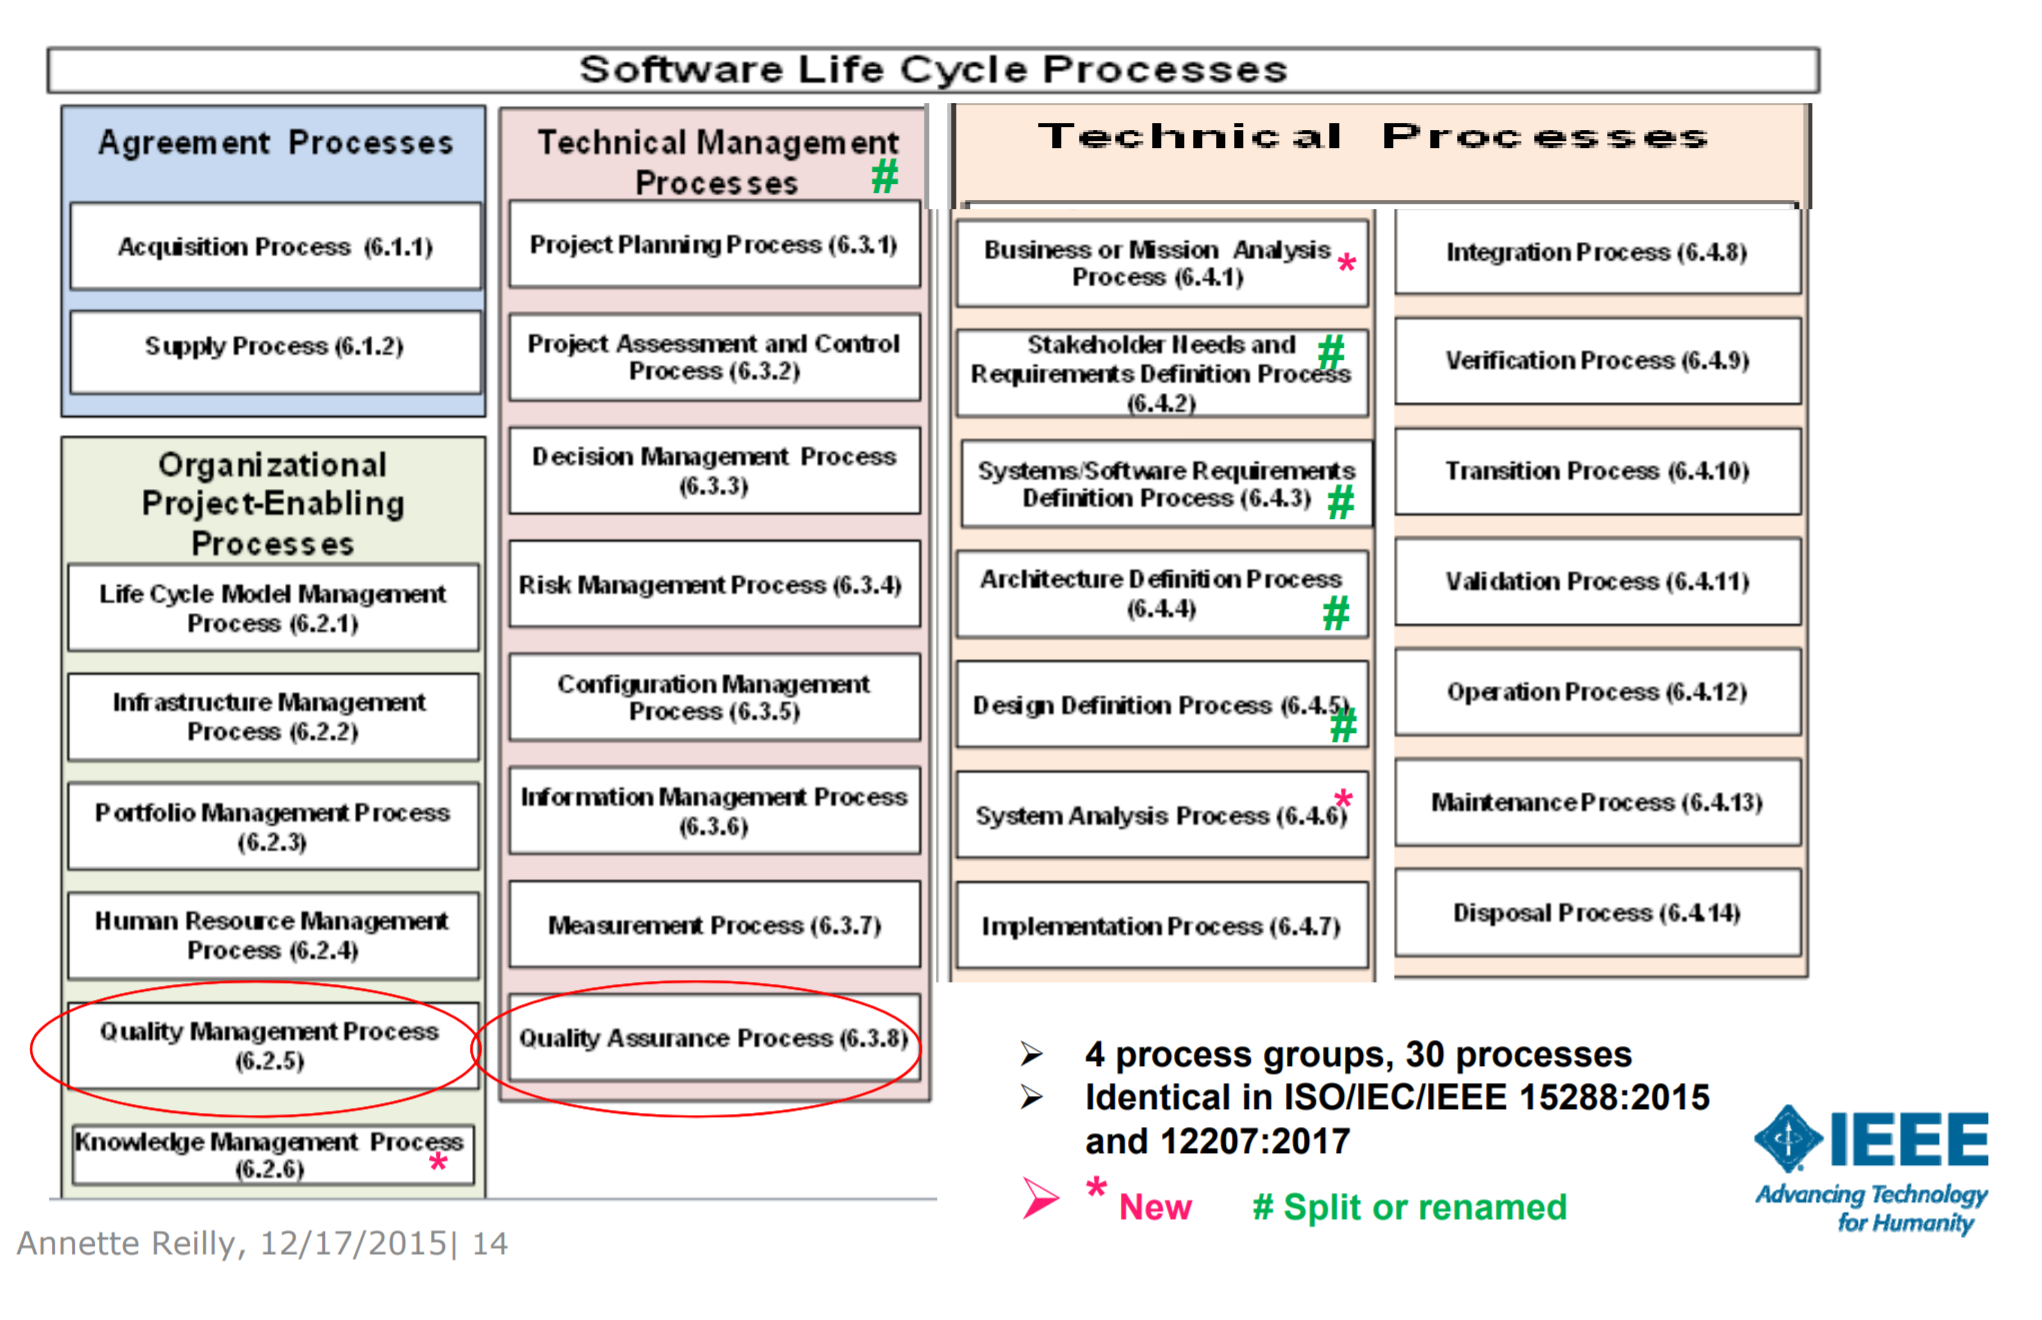
\includegraphics[scale=0.7]{ISO12207:17}
\end{center}
\section{Process Implementation}
\begin{itemize}
	\item Define or select software life cycle model appropriate to the scope, magnitude, and complexity of the project;
	\item Select, tailor, and use standards, methods, tools, and programming languages (if not stipulated in  contract);
	\item Develop plans for conducting the activities of the Development process.
\end{itemize}
\section{ISO 15504}
Process assessment: What is it?
\begin{itemize}
	\item A disciplined examination of the processes by an organisation against a set of criteria to determine capability of those processes to perform within quality, cost and schedule goals
	\item Focus here is on continual, self-improvement
\end{itemize}
Why bother?
\begin{itemize}
	\item Identify strengths and weaknesses in current utilisation of processes
	\item Ongoing development of systems, maturity and growth
	\item Feeds into the future
\end{itemize}
\begin{center}
	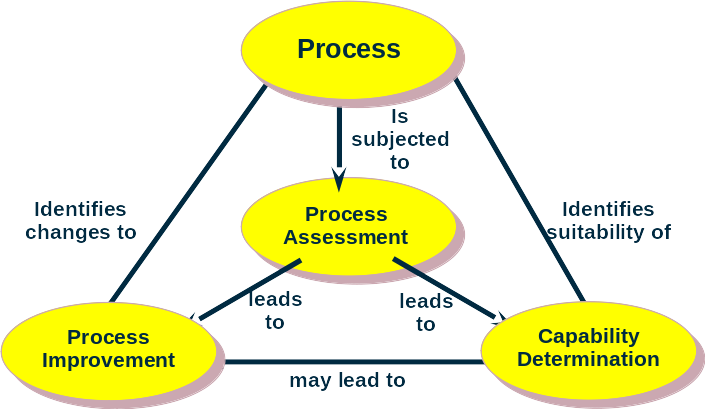
\includegraphics[scale=0.7]{ISO15504}
\end{center}




\end{document}